\chapter{Literature review}
\label{LR}

\section{Phage Biology}
\subsection{What Are Phages?}
Phages are small bundles of proteins that contain viral DNA. 
Phages are composed of multiple parts, built like LEGO blocks, to complete the task of infecting a bacterium. 
\Cref{fig:figures:phage_diagram} shows the body parts of a phage. 
The phage aims to find a suitable bacterial host and infect the host with viral DNA. 
The DNA alters the host’s metabolic pathways to its benefit and hijacks the cellular replication process to create new copies of the phage. 
Eventually, the cell lyses, releasing the newly created phages into the environment to infect more bacteria. 
\begin{figure}[h!]
    \centering
    \begin{subfigure}{0.25\linewidth}
        \centering
        \captionsetup{width=1\linewidth}
        \includegraphics[width=\linewidth]{Figures/phage_diagram.png}
        \caption{
            Phage body structure. 
            Image sourced from \citet{FlatIllustrationBacteriophage}. 
        }
        \label{fig:figures:phage_diagram}
    \end{subfigure}
    \hfill
    \begin{subfigure}{0.3\linewidth}
        \centering
        \captionsetup{width=1\linewidth}
        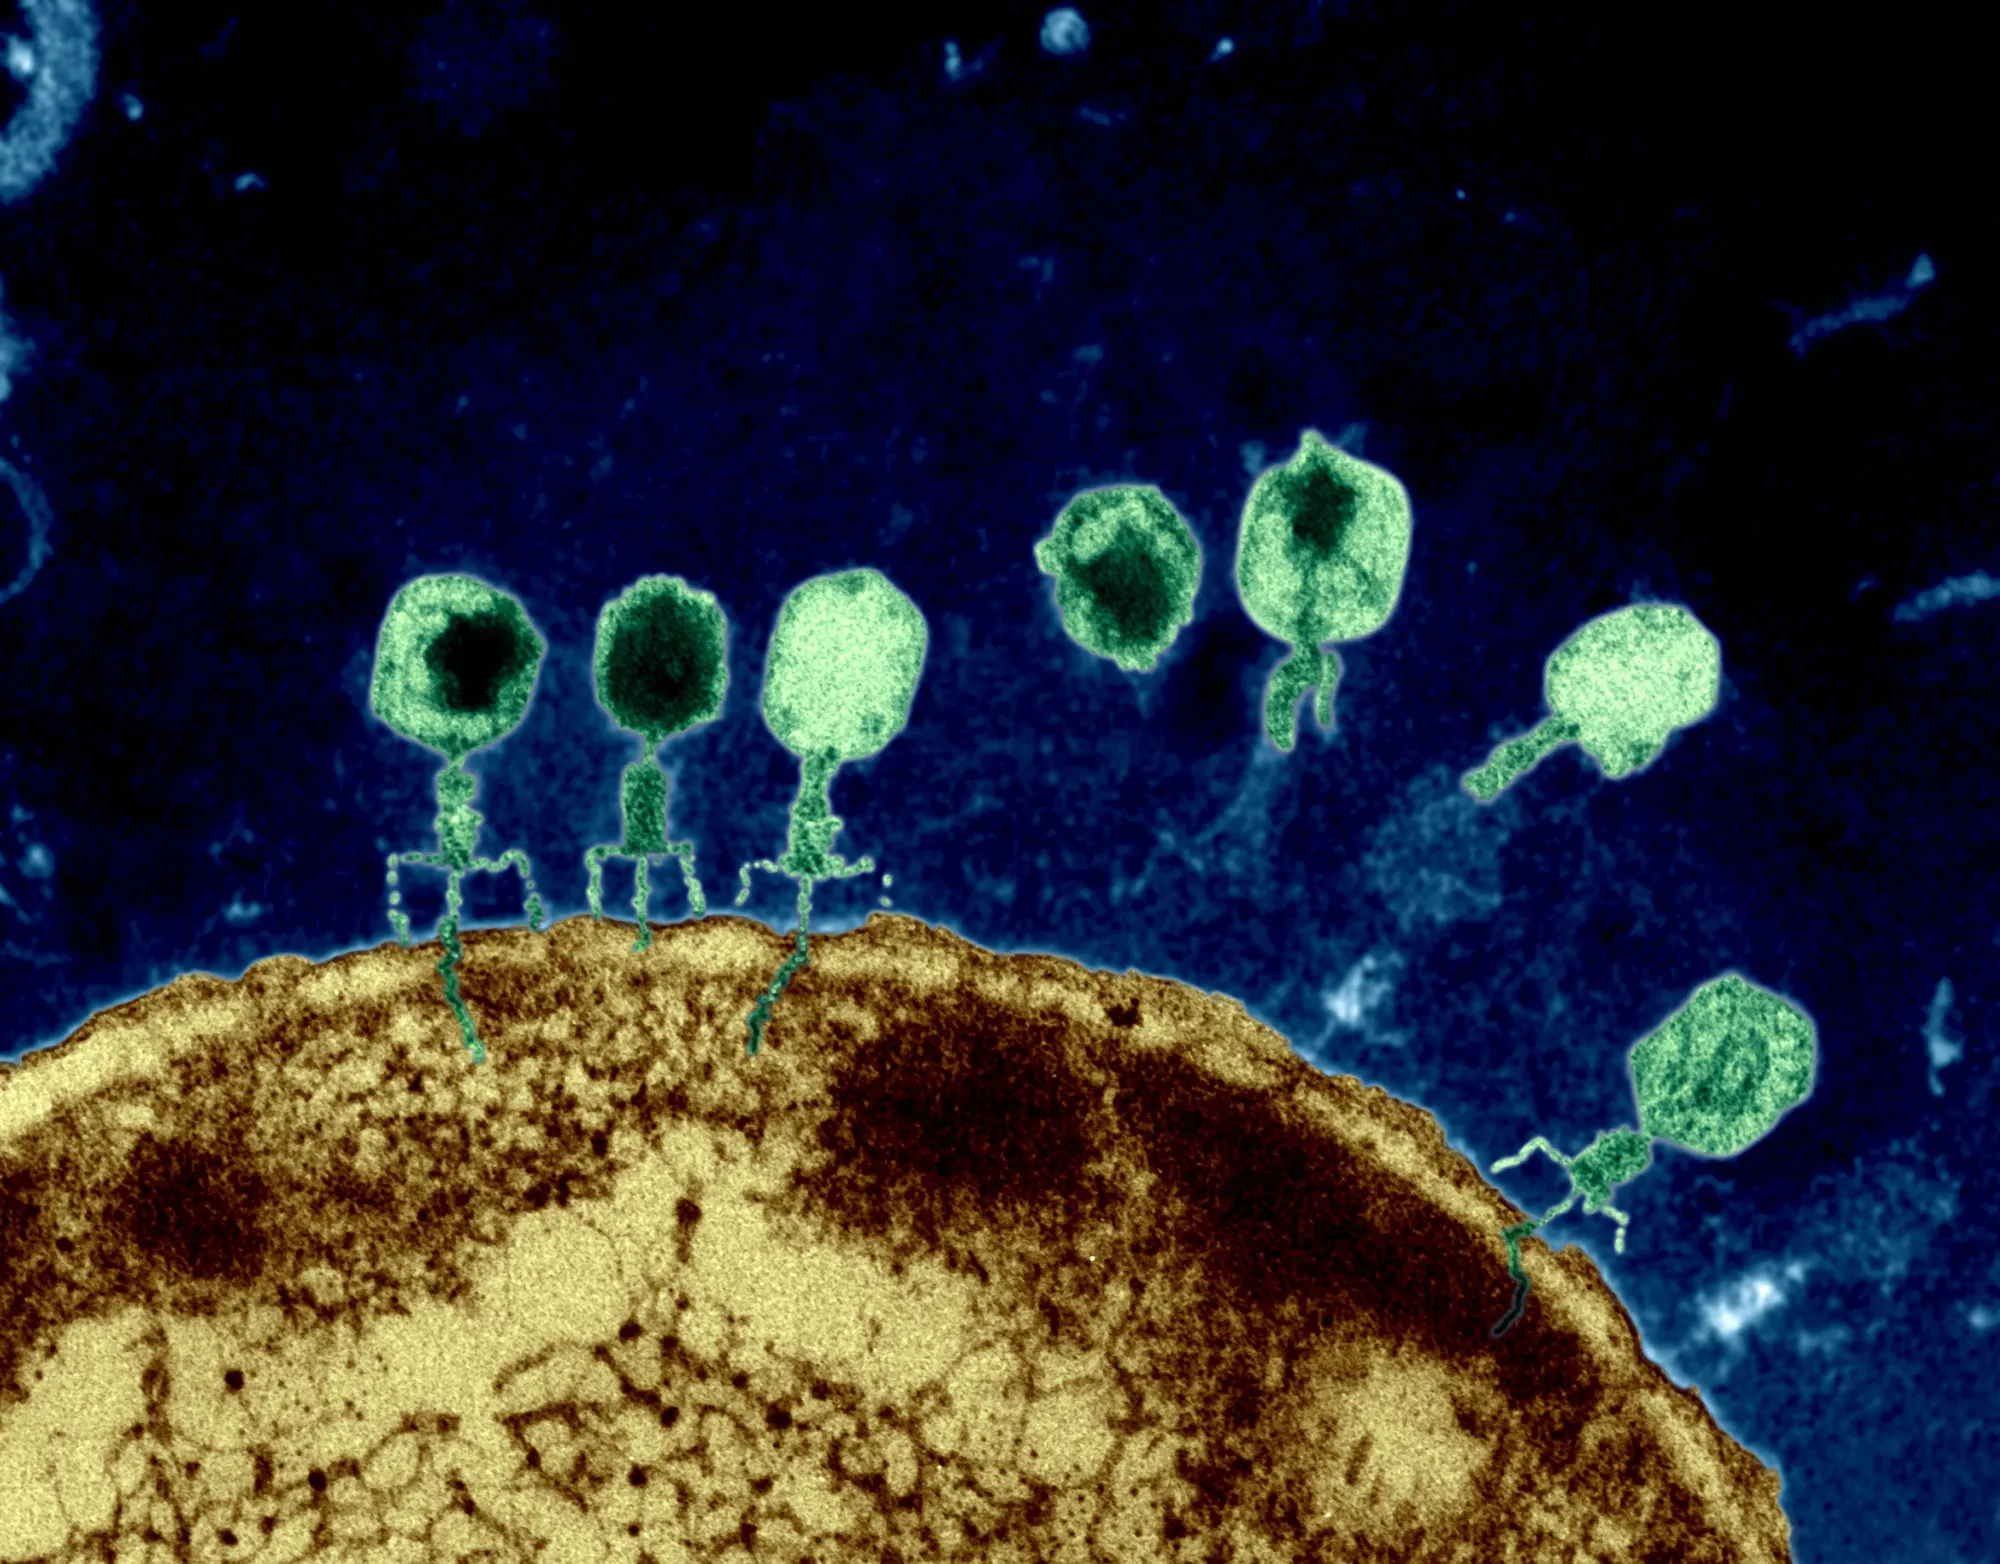
\includegraphics[width=\linewidth]{Figures/phage_real.png}
        \caption{
            Phages infecting an \textit{E. coli} bacteria. 
            Image sourced from \citet{twilleyWorldViralDark2015}. 
        }
        \label{fig:figures:phage_real}
    \end{subfigure}
    \hfill
    \begin{subfigure}{0.35\linewidth}
        \centering
        \captionsetup{width=1\linewidth}
        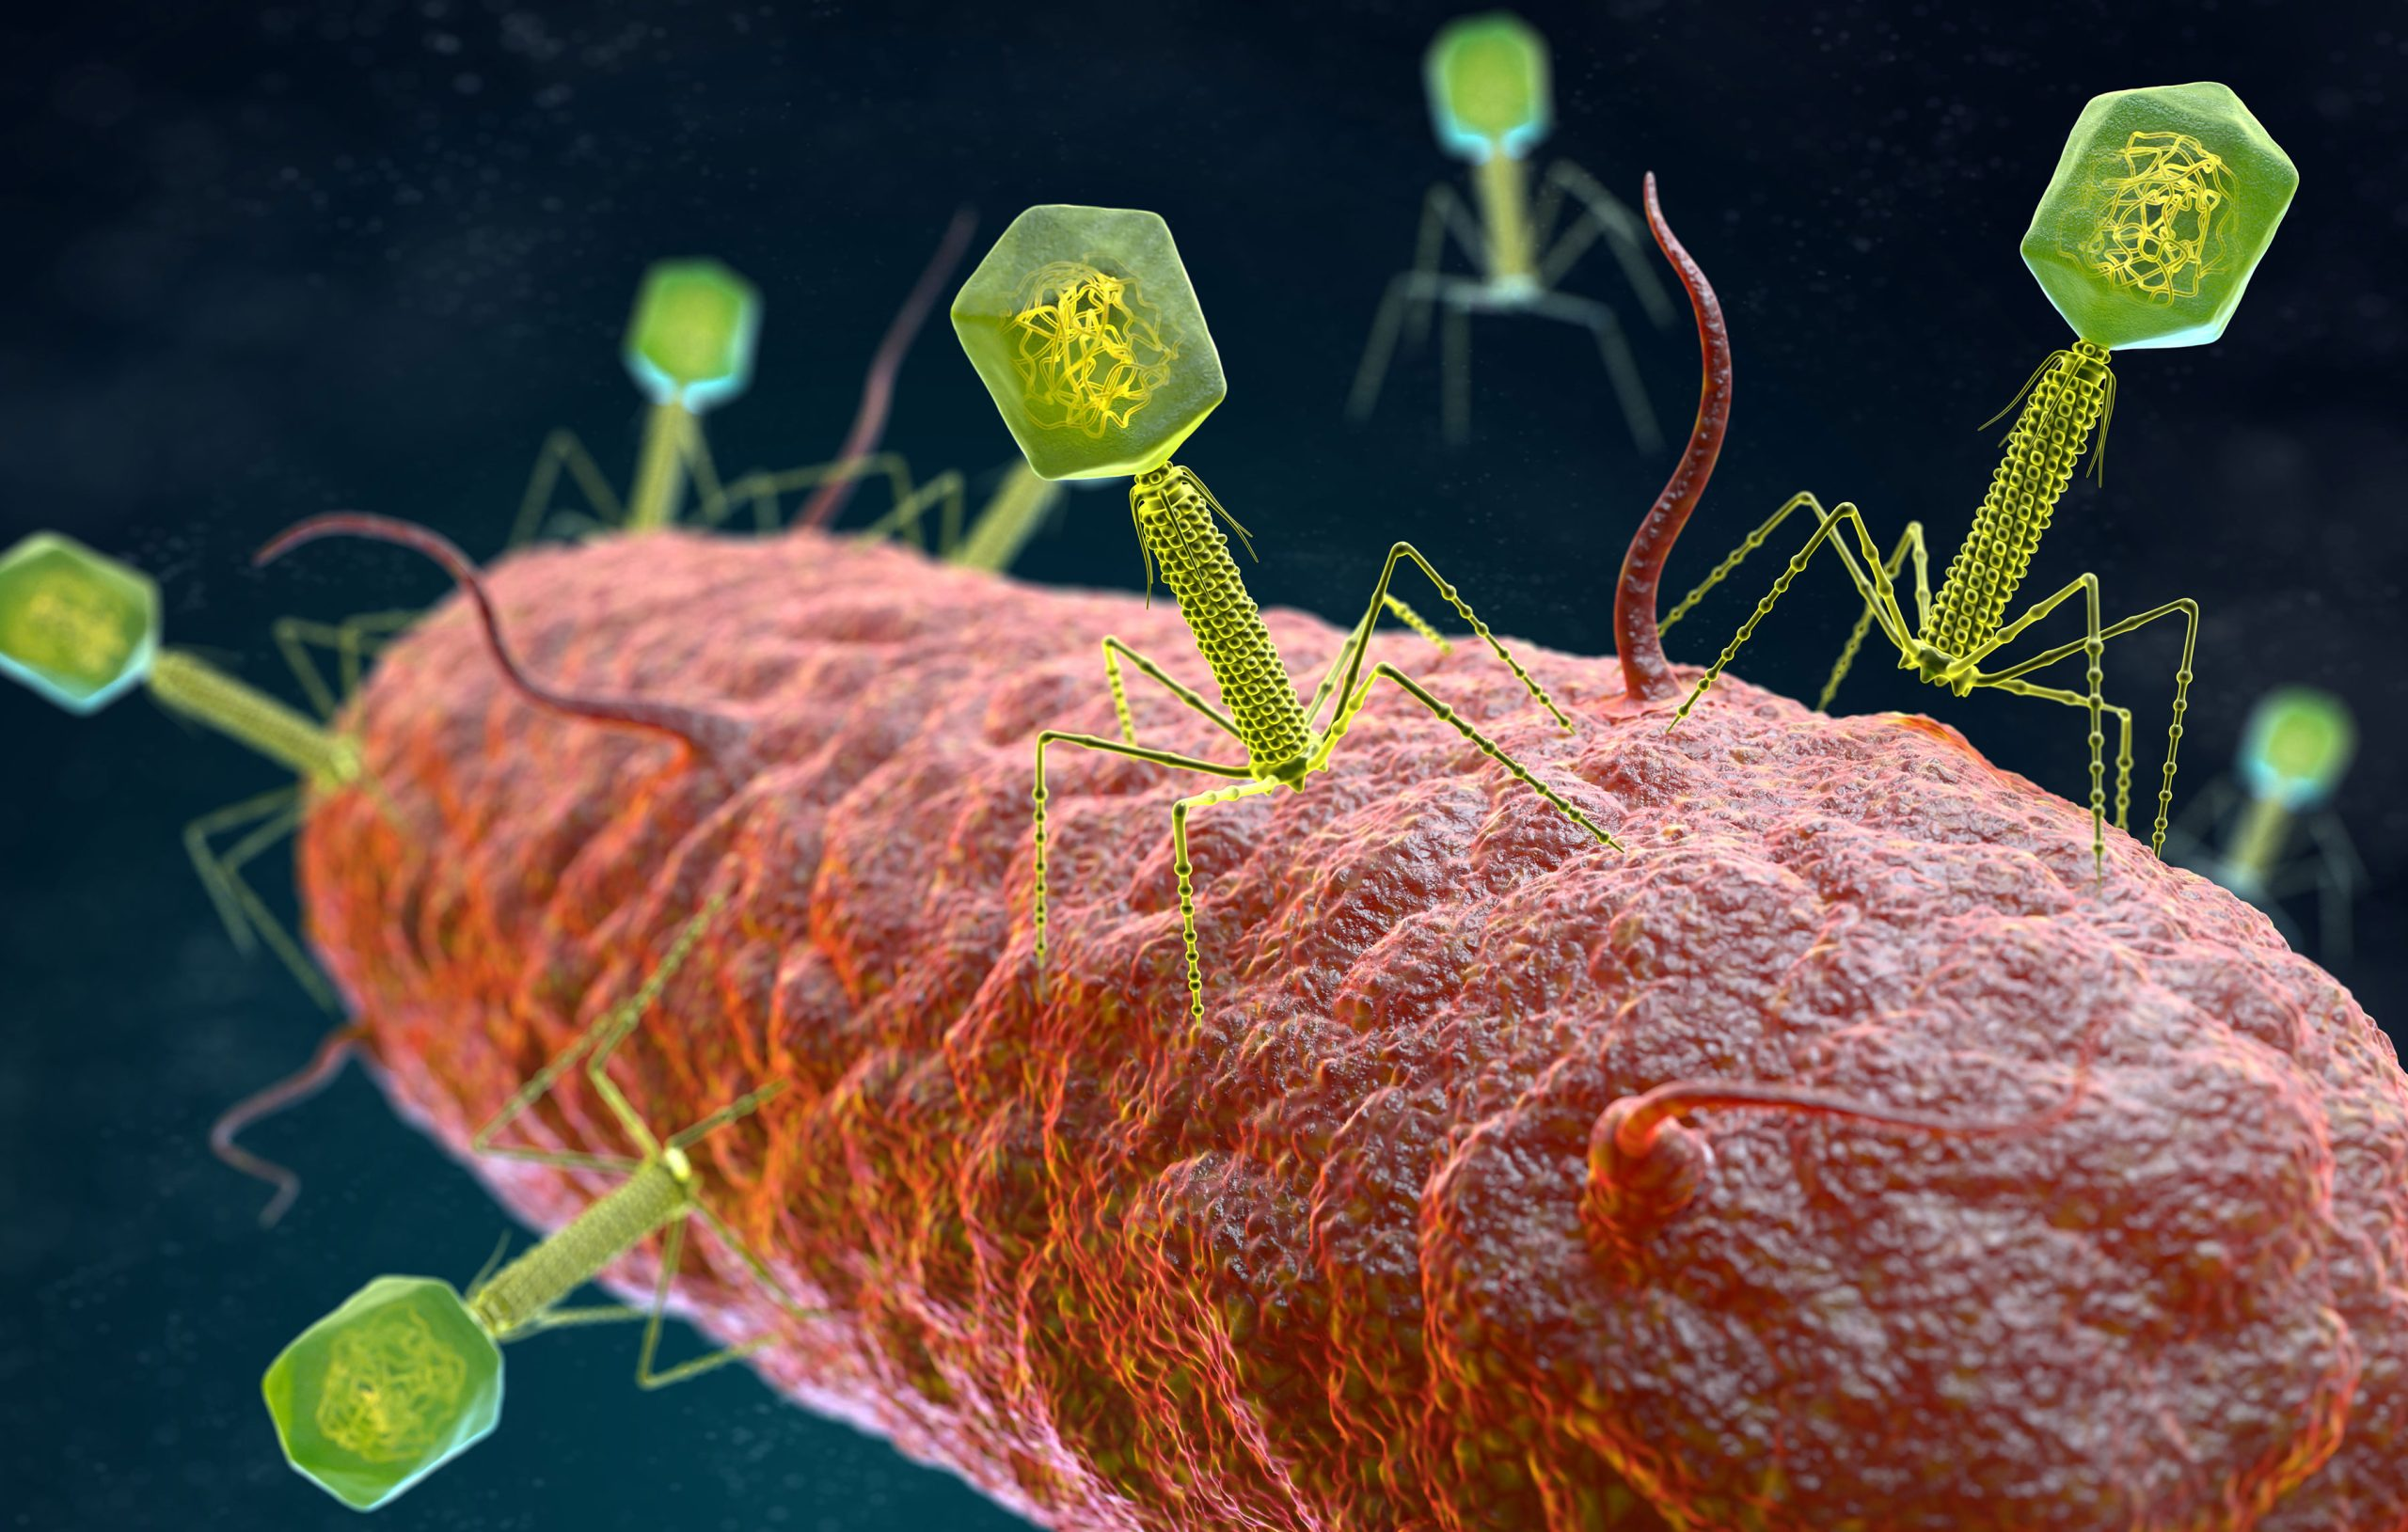
\includegraphics[width=\linewidth]{Figures/phage_impression.png}
        \caption{
            Artist representation of phages infecting a bacterium. 
            Image sourced from \citet{VirusesMayPlay} 
        }
        \label{fig:figures:phage_impression}
    \end{subfigure}
    \caption{Parts of a phage, a real-life picture of phages infecting an \textit{E. coli} bacterium, and an artist’s impression of phages infecting a bacterium. }
\end{figure}

\subsection{How Does the Phage Cycle Work?}
There are three main parts to the phage-bacteria host cycle: the infection stage, the lysogenic cycle, and the lytic cycle. 
\Cref{fig:phage_life_cycle} shows an overview of the phage cycle. 

In the infection stage, a phage attaches to the surface of a bacteria cell. 
The infection stage involves the phage searching for, detecting, and attaching to a bacterium, followed by the injection of its DNA into the bacterium. 
Detection and attachment occur via phage receptor-binding proteins located at the tip of the phage tail that recognize specific receptors on the bacterial cell wall, triggering conformational changes that enable DNA injection \cite{lindbergBacteriophageReceptors1973}. 
The success of this process depends on the specificity and density of both phage and bacterial receptors \cite{stoneUnderstandingExploitingPhage2019}. 
Once attached, the phage injects its DNA into the host cytoplasm, where it can replicate independently.
Once injected, the phage-cell pair enters either the lysogenic cycle or the lytic cycle. 

The lysogenic cycle involves phage DNA integrating into the bacterial genome as a prophage, where it is replicated along with the host cell without causing immediate lysis.
The phage evades host defenses such as CBASS and CRISPR-Cas systems, which can initiate programmed cell death, preventing phage replication or detect and degrade foreign DNA \cite{banhBacterialCGASSenses2023, levyCRISPRAdaptationBiases2015}. 
Programmed cell death helps recycle resources for other bacteria \cite{warwick-dugdaleHosthijackingPlanktonicPiracy2019}. 
Once integrated, the prophage can alter host fitness and provide resistance to other phages. 
During cell division, the prophage is copied into daughter cells but remains at risk of being excised by restriction enzymes \cite{sharpMolecularEvolutionBacteriophages1986}.
Under certain stress conditions, such as DNA damage or activation of the SOS response, the prophage induces itself to exit the genome and enter the lytic cycle \cite{waldorPhageRegulatoryCircuits2005, stoneUnderstandingExploitingPhage2019, fortierImportanceProphagesEvolution2013}.

The lytic cycle is the process where a phage infects a bacterium, hijacks its replication machinery to produce new phage components, assembles these parts, and ultimately lyses the host cell to release new phages. 
This process involves hijacking the host’s DNA replication to synthesize phage parts like the capsid, sheath, and tail (\Cref{fig:figures:phage_diagram}). 
The phage does this by redirecting resources from internal cellular functions towards viral replication \cite{warwick-dugdaleHosthijackingPlanktonicPiracy2019}. 
The parts self-assemble via protein-protein and protein-nucleic acid interactions \cite{aksyukBacteriophageAssembly2011}. 
Phages induce bacterial lysis by producing holin proteins that disrupt the cell membrane, releasing the phages and resources \cite{wangHolinsProteinClocks2000}.

\section{Bacterial Defense Against Phages} 
\label{sec:literaturereview:bacterial_defense_against_phages}
There is a constant battle between phages and bacteria. 
The bacteria do not want to be killed by the phages, so they develop defenses such as thickening their cell walls or destroying the viral DNA. 

\subsection{Mutations in Bacterial DNA (Genetic (Co-)Evolution)}
As bacteria cells grow and divide, random point mutations can occur in the DNA. 
These mutations can affect phage defenses, like thickening the cell wall or removing a receptor, making it harder for the phages to detect and infect the cell. 
Mutations can be partially effective if full effectiveness requires multiple steps to achieve. 
Random mutations can also fail to make the bacteria more resistant to phages by increasing phage susceptibility or by incurring a cost to the bacterial cell, such as losing receptors on the cell wall \cite{lenskiTWOSTEPRESISTANCEESCHERICHIA1984}. 

\subsection{Horizontally Transferring DNA}
Bacteria can horizontally transfer DNA to other bacteria on contact. 
A donor cell can donate DNA fragments using a mechanism called a pilus. 
The pilus acts as a tunnel between the donor cell and the recipient cell so that DNA can transfer from the donor cell to the receiver cell \cite{harbSsRNAPhagePenetration2020}. 

A phage can accidentally collect a piece of the host’s DNA instead of its DNA during assembly. 
The phage, with the now dead host’s DNA, can infect the next bacterium, injecting the new bacterium with the dead cell’s DNA, thereby horizontally transferring the DNA \cite{tamangHorizontalGeneTransfer2023, kasmanBacteriophages2025}. 
The transferred DNA can include natural phage defenses or alter the bacterium’s genes and phenotype, making it undetectable to future phages. 

\subsection{Phage Inactivation and Decoys}
Bacteria can further protect themselves by producing decoys that the phage will attach to rather than themselves. 
Freshly lysed bacteria may still have biomarkers that attract phages, leading phages to attach to non-viable cells where successful infection cannot occur.
Bacteria can also produce proteolytic enzymes that will damage the proteins found in a phage \cite{tanQuorumSensingDetermines2015}. 
Some bacteria can produce outer membrane vesicles that phages can absorb to, and later detach and float away with the phage \cite{rabinovitchBacterialDebrisEcological2003}. 
These vesicles are suspected of having a minor impact as a sink \cite{bullPhageBacterialDynamicsSpatial2018}. 
\citet{deyEmergentHigherorderInteractions2025} showed that these vesicles, a “debris” term for the phages, had a positive effect on coexistence in large phage-bacteria communities. 

\subsection{Phenotype Resistance}
Not all new phenotypes arise from genetic mutations. 
Resistance can result from phenotypic variation within a genetically identical population, allowing bacteria to express different resistance traits without altering their DNA.
\citet{guptaCombinatorialPhenotypicLandscape2025} found that some \textit{Bacteroides fragilis} bacteria were able to evade phage infection.  
The presence of combinatorial phenotypic states, where the differential expression of protective mechanisms created rare, super-resistant cells capable of withstanding phage attack.
By acting together, these heterogeneously expressed anti-phage defense mechanisms created a phenotypic landscape where distinct protective combinations enabled the survival and re-growth of bacteria expressing these phenotypes without acquiring additional mutations \cite{guptaCombinatorialPhenotypicLandscape2025}. 

\subsection{Spatial Refuge/Biofilms} 
Bacteria can evade phages by forming spatial refuges, such as biofilms, or hide behind physical structures. 
Biofilms are dense microbial communities embedded in mucus, which impedes phage diffusion and protects resident bacteria \cite{abedonPhageDelayEnhancing2017}. 
On agar plates, spatial structure similarly limits phage spread \cite{eriksenGrowingMicrocolonyCan2018}. 
While phages rely on passive diffusion, bacteria can actively move, further enhancing their survival \cite{lohrmannInfluenceBacterialSwimming2024}.

\section{Phage Counter Defense Against Bacteria}
With some of the defenses that bacteria have developed, phages are constantly mutating to counter their defenses. 
If phages do not adapt to the ever-changing bacterial defenses, the phages will die out due to their inability to infect and multiply. 
It becomes an arms race, with each side trying to out-adapt the other. 
The bacteria and phages must have a delicate balance to ensure coexistence. 

\subsection{Genetic Mutations}
Mutations in viral DNA will affect how the phage body parts are designed and built. 
These mutations will affect both external phage behavior, such as how it detects a bacterium, and internal behavior, including evading detection and integrating with the cell’s DNA. 
The changes will lead to changes in overall phage fitness, i.e., the ability of the phage to infect, replicate, and lyse bacteria. 

\subsection{Viral Recombination}
Multiple phages can infect a cell and replicate itself using the cell’s internal replication process. 
Each phage has unique building blocks, including the capsid, tail, and sheath. 
If the proteins that build the subparts of each phage have similar chemical properties, the phage parts can be swapped between phages \cite{aksyukBacteriophageAssembly2011}. 
The swapping of parts allows for biological diversity to spread throughout a phage population. 
Each phage body part can have unique characteristics, such as a higher attachment rate, a larger DNA storage capsule, or a better probability of injection. 

\section{Phage Defense Against Phages}
Some phages can employ defenses against other phages from infecting the bacterial cell, ensuring that the host’s resources are all for itself. 
The act of preventing a secondary infection from a similar or closely related phage is called superinfection exclusion (SIE) \cite{patelAntiphageDefenceInhibition2024}. 
The following are several methods for preventing further infections. 

\subsection{Altering Cell Structure}
The prophage can alter the surface receptors of the bacteria, making it harder for other phages to detect the bacteria, reducing the chance of attachment and injection by other phages \cite{bucherPhageMachineSIEence2024}. 

\subsection{Protein Creation}
Other phages, like the T4 phage, can create proteins like the Spackle protein, which inhibits the lysozyme activity used in the process of DNA injection by other phages \cite{bucherPhageMachineSIEence2024, kanamaruStructureFunctionT42020}. 
Some prophages can encode proteins that will interfere with the replication process of other phages. 
For example, the SieA protein encoded by phage P22 blocks infection from other phages \cite{leavittBacteriophageP22SieAmediated2024}. 

Tail Assembly Blocker (TAB) is an anti-phage defense mechanism encoded by a \textit{Pseudomonas aeruginosa} prophage. 
While TAB permits the invading phage to replicate its genome, it inhibits the assembly of the phage tail, thereby preventing the production of infectious virions. 
The prophage that encodes TAB is not affected by this inhibition, as it also expresses a protein that neutralizes TAB’s blocking activity. 
Although the host cell still undergoes lysis, no infectious phages are released.

\section{Bacteria and Phages in the Lab}
Researchers worldwide are conducting laboratory experiments to gain a deeper understanding of the interactions between phages and bacteria. 
The aim is to gain a better understanding of how phages work and interact with bacteria at the molecular, host, and population levels. 

\subsection{Running Experiments}
Laboratory experiments are often conducted in a liquid medium containing the necessary resources for bacterial growth. 
This liquid medium, often referred to as broth, facilitates the cultivation of bacteria in a well-mixed environment, allowing researchers to monitor bacterial growth and phage infection dynamics over time. 
By adjusting parameters such as resource concentration, temperature, and pH, researchers can simulate different environmental conditions and observe their effects on phage-bacteria interactions. 

Samples are collected at set time points to measure bacterial density, phage titer, and resource concentration. 
These data enable researchers to fit mathematical models, estimate growth rates, and determine phage parameters, such as latent time and burst size, from one-step growth curves \cite{gengUsingBacterialPopulation2024, mullaExtremeDiversityPhage2024}.

\subsection{Chemostats}
Commonly used setups include those containing liquids with phages, bacteria, and resources in a chemostat and in batch culture. 
Chemostats enable the continuous addition of resources and removal of waste, thereby maintaining steady-state conditions that are ideal for studying long-term dynamics.

\subsection{Petri Dishes}
Petri dishes are another common method used to grow bacterial colonies. 
Agar, a jelly-like substance derived from seaweed, is commonly added to create a solid growth medium in Petri dishes. 
Agar provides a stable surface for bacteria to grow on and form visible colonies. 
Clear zones, known as plaques, appear where phages have infected and lysed the bacteria, enabling the quantification and observation of phage activity. 
The phages can diffuse on the agar plate, infecting neighboring cells. 
Phage infection creates clear plaques (2-3 mm) where bacteria are absent. 
\Cref{fig:phage_petri_dish} shows an example of a bacteria lawn with phage plaques. 

\subsection{Measuring Growth}
Bacterial density in liquid media is usually measured by optical density (OD) using a spectrophotometer. 
OD measurements require calibration and are not directly comparable across devices \cite{bealRobustEstimationBacterial2020}. 
Using cell counts (e.g., $cells/ml$) allows for more consistent comparisons across experiments and labs \cite{miraEstimatingMicrobialPopulation2022}.

With Petri dishes, it is more challenging to measure bacterial growth and plaque size accurately. 
It may be possible to wash the bacteria off into a test tube with water to measure the optical density, but the results are inconsistent. 
It may be possible to quantify the change in plaque size using an image analysis program; however, the results may be inaccurate and sensitive to variations in lighting conditions. 

\begin{figure}[h!]
    \includegraphics[width=0.5\textwidth]{Figures/phage_petri_dish.jpeg}
    \centering
    \caption{
        Bacteria lawn, the dots on the petri dish show no bacteria growth due to the presence of phages. 
        Photo courtesy of S. Flickinger. 
    }
    \label{fig:phage_petri_dish}
\end{figure}

\subsection{Serial Transfer}
Serial transfer (ST) is a method employed by a bacteriologist, where, after a set amount of time, the bacteriologist pipettes medium containing phages, bacteria, and resources out of a test tube and adds the old medium to a new test tube with fresh medium.
At this stage, the bacteriologist can add more bacteria or phages to the test tube. 
Only resources are typically added during the transfer process. 
Researchers can optically measure bacterial density using an optical density meter or employ a mass spectrometer to determine phage concentration at set time points during the experiment. 
As the bacteria grow, they consume the resources found in the medium.
The resources will eventually run out, and the bacteria die out due to a lack of resources.
By introducing new resources at set time intervals, the bacteria can regrow and exhibit a semi-stationary behavior.

\subsection{Growth Curves Typically Seen in a Lab}
\label{sec:literaturereview:growth_curves_typically_seen_in_a_lab}
When choosing model parameter values, it is essential to select values that can realistically be found in real-life systems and be replicated in the lab. 
Various features characterize a growth curve produced in a lab that a model should aim to reproduce. 

The idealized dynamics of bacterial populations undergoing phage infection have several phases. 
First, there is an apparent exponential rise in bacteria growth, growing 40-100x in population in the span of a few hours. 
At a certain point in time, the bacterial population starts decreasing almost as fast as it was growing. 

Phage populations also exhibit exponential growth but with a delay in growth relative to the bacterial population. 
Initially, there was no growth in the phage population. 
After a set amount of time, the phage population will start to grow and peak a few hours after the bacteria population reaches its peak. 
If there is no phage death or removal, the phage population will eventually reach a plateau when every bacteria has died. 

\Cref{fig:created:a_good_curve_linear} shows an example of a curve for a $1\times1\times1$ system that would typically be seen in a lab. 
\Cref{fig:created:a_good_curve_logarithmic} is the same plot but with a logarithmic y-axis. 
These specific plots exhibit a clear growth, peak, delay, and death cycle. 

\begin{figure}[h!]
    \centering
    \begin{subfigure}{1\linewidth}
        \centering
        \captionsetup{width=1\linewidth}
        \includegraphics[width=\linewidth]{Plots/Created/a_good_curve_linear.png}
        \caption{
            An example linear y-axis for a curve that researchers aim to replicate. 
        }
        \label{fig:created:a_good_curve_linear}
    \end{subfigure}
    \hfill
    \begin{subfigure}{1\linewidth}
        \centering
        \captionsetup{width=1\linewidth}
        \includegraphics[width=\linewidth]{Plots/Created/a_good_curve_logarithmic.png}
        \caption{
            The equivalent logarithmic y-axis plot for a curve that researchers aim to replicate. 
        }
        \label{fig:created:a_good_curve_logarithmic}
    \end{subfigure}
    \caption{
        Growth of a population in a $1\times1\times1$ system. 
        The log plot allows us to visualize behavior at values approaching zero and to plot data on a logarithmic scale. 
        The parameters used for this plot can be found in \Cref{tab:appendixE:a_good_curve}. 
    }
    \label{fig:created:a_good_curve}
\end{figure}

\section{Software Mathematically Modelling Phages, Bacteria, and Resources}
Some software programs modeling phage-bacteria-resource interactions already exist. 
Here, I cover three software programs, Cocktail, PhageDyn, and PhiSite, that have been created to model phages and bacteria, as well as their limitations. 

\subsection{Cocktail}
\citet{nilssonCocktailComputerProgram2022} developed Cocktail to model phage-bacteria-resource kinetics in a chemostat. 
The model assumes that phage A, phage B, and the combination of both phages (phage AB) can simultaneously infect a single bacterial strain. 
The model simulates bacterial resistance to phage A and phage B, as well as a combination of phage A and B. 
The user can control parameter values, such as resistance rates to A, B, and AB, resource concentration and outflow, and phage adsorption rate. 
The user can also control model settings, such as if the model is deterministic or stochastic, and the step size \cite{nilssonCocktailComputerProgram2022}. 
\Cref{fig:sourced:cocktail_plot} shows four sample output plots. 

\subsection{PhageDyn}
PhageDyn, developed by \cite{krysiak-baltynSimulationPhageDynamics2017}, is a Java applet that models phage dynamics in multi-reactor industrial wastewater treatment plant models. 
PhageDyn interacts with existing GPS-X \cite{AdvancedWastewaterModelling} files to incorporate phage dynamics into models of industrial wastewater treatment plants. 
\citet{krysiak-baltynSimulationPhageDynamics2017} developed PhageDyn to determine how phages can reduce foaming caused by bacteria in wastewater treatment plants, another real-life application of phages \cite{heardEffectFilamentousBacteria2008}. 
PhageDyn does not simulate phage dynamics on its own; instead, it manipulates existing files in GPS-X to incorporate phage dynamics into wastewater treatment plant models. 
\Cref{fig:sourced:phagedyn_plot} shows the output that PhageDyn provides. 

\subsection{PhiSite}
PhiSite is a website created by \citet{bekeModellingInteractionBacteriophages2016} to allow users to interact with the \citet{schragHostParasiteCoexistenceRole1996} model. 
The website can be accessed \href{http://dublin.embnet.sk:3838/model/}{here}. 
It is possible to adjust various input parameters, such as the temperature and pH of the system, the infected bacteria count, washout, and more. 
It is possible to download the graphs and raw simulation data from the dashboard.
See \Cref{sec:lit:schrag} for more details on the model. 
\Cref{fig:sourced:phisite_plot} shows the output that PhiSite provides. 

\subsection{Cocktail, PhageDyn, and PhiSite Limitations}
\label{sec:literature:cocktail_and_phagedyn_limitations}
There are limitations to all three software. 
Cocktail can model up to a $2\times 1 \times 1$ system and in a chemostat environment. 
Chemostats receive a constant influx of new resources and a constant removal of medium from the chemostat. 

Cocktail’s ODE model is not readily adaptable to other model equations.
The ODE model accepts inputs from a hardcoded GUI front end. 
Any changes to the front end or the ODE model will require corresponding changes to both the ODE model and the front end to accommodate the new inputs and outputs. 
The code for Cocktail is open source, so adding new buttons and modifying the model should not pose a significant challenge, but it is still a considerable undertaking. 

PhageDyn is used with GPS-X, a highly specialized wastewater treatment modeling software. 
PhageDyn is programmed for a specific task, with no flexibility in modifying the model or inputs. 
PhageDyn assumes biomass instead of individual bacteria populations. 
However, PhageDyn is no longer available for download.

PhiSite faces similar limitations to Cocktail, where the model input is hard coded to the front end, making it difficult to change the ODE model inputs and challenging to run multiple simulations simultaneously to cover a wide range of parameter values. 
There is no built-in method to programmatically iterate over a set of values and download the data. 
The data needs to be downloaded individually and then combined into a graph. 

\begin{figure}
    \centering
    \begin{subfigure}{0.32\linewidth}
        \centering
        \captionsetup{width=1\linewidth}
        \includegraphics[width=\linewidth]{Plots/Sourced/cocktail_plot.png}
        \caption{
            Figure A) \textit{E. coli} infected with phage T4 in a chemostat exhibiting an oscillating growth behavior, following the model of \citet{bohannanEffectResourceEnrichment1997}. 
            Figure B) Oscillations of bacteria and phages can exist at higher titers, dependent on low resource concentration, following the model of \citet{lenskiDynamicsInteractionsBacteria1988}. 
            Figure C) As the concentration of resources change, this results in increasing oscillations, but not going extinct. 
            Figure D) A system modeling the interactions with phage A and B. 
            Figure and caption sourced from \citet{nilssonCocktailComputerProgram2022}. 
        }
        \label{fig:sourced:cocktail_plot}
    \end{subfigure}
    \hfill
    \begin{subfigure}{0.32\linewidth}
        \centering
        \captionsetup{width=1\linewidth}
        \includegraphics[width=\linewidth]{Plots/Sourced/phagedyn_plot.png}
        \caption{
            \textcolor[HTML]{551A8C}{\textbf{Purple}} is heterotrophic biomass, 
            \textcolor[HTML]{4580B4}{\textbf{Blue}} is foaming biomass, 
            \textcolor[HTML]{FF0000}{\textbf{Red}} is phages, 
            \textcolor[HTML]{01E6EE}{\textbf{Light Blue}} is total suspended solids. 
            Figure A) Biomass concentration immediately post phage dosing. 
            Figure B) Biomass concentration with low phage concentration and maintain low concentration post spike in population count. 
            Figure C) Biomass concentration when phages are extinct. 
            Figure D) Biomass concentration with a less virulent and low adsorption rate phage, indicating coexistence with biomass. 
            A change in phage concentration shows a decrease in heterotrophic and foaming biomass \cite{krysiak-baltynSimulationPhageDynamics2017}. 
            Figure and caption sourced from \cite{krysiak-baltynSimulationPhageDynamics2017}
        }
        \label{fig:sourced:phagedyn_plot}
    \end{subfigure}
    \hfill
    \begin{subfigure}{0.32\linewidth}
        \centering
        \captionsetup{width=1\linewidth}
        \includegraphics[width=\linewidth]{Plots/Sourced/phisite.png}
        \caption{
            Running the simulations under five different conditions.
            The simulations have been run under different conditions to demonstrate the capabilities of the designed model. To set up the simulation the values of maximal, minimal and the optimal pH and temperature have to be experimentally stipulated. 
            Then the model can calculate specific growth rate under different pH and temperature. 
            Figure and caption sourced from \citet{bekeModellingInteractionBacteriophages2016}
        }
        \label{fig:sourced:phisite_plot}
    \end{subfigure}
    \caption{
        Example output from Cocktail, PhageDyn, and PhiSite, respectively. 
        For PhageDyn, the concentration of heterotrophic biomass in an aerobic plug flows across four situations.
        See \citet{nilssonCocktailComputerProgram2022}, \citet{krysiak-baltynSimulationPhageDynamics2017}, and \citet{bekeModellingInteractionBacteriophages2016} for more information on parameter values and supplementary resources. 
    }
    \label{fig:sourced:cocktail_and_phagedyn}
\end{figure}

\section{Methods of Modeling Phages and Bacteria}
There are various ways to model phage, bacterial, and resource populations and their interactions; however, the most common approach is to use Ordinary Differential Equations (ODEs) or Delay Differential Equations (DDEs). 

The ODE method is simple to understand and easy to set up, but it can only capture large population dynamics.
Certain assumptions about community interactions also need to be made, such as the assumption that everything is probabilistic.
For example, every timestep, $\alpha$ percentage of phages interact with  bacteria
DDEs are similar to ODEs, but DDEs incorporate time delays to account for processes that depend not only on the current state but also on past states, thereby incorporating behavior that has a delay, such as latent infection time. 

One way to introduce a delay in the infected bacteria releasing phages is to force the infected bacteria to undergo a series of stages. 
Once the infected bacterium has progressed through every stage of infection, it releases the phages into the system. 
For example, in the paper \citet{gengUsingBacterialPopulation2024}, infected bacteria go through $M$ stages of infection before lysing. 
By decreasing $\tau$ (the latent period) in the model proposed by \citet{gengUsingBacterialPopulation2024}, more infected bacteria go from infected state $i$ to infected state $i+1$ per timestep with rate $\frac{M}{\tau}$, causing the infected peak population count to peak earlier. 
 
Each model can be further developed, for example, by adding temperature and pH dependence, bacteria releasing nutrients upon lysis, or phage resistance. 

\subsection{Campbell DDE Model for Chemostats}
The \citet{campbellConditionsExistenceBacteriophage1961} model is a DDE model that describes the growth of bacteria and phages in a chemostat, a bioreactor used to cultivate microorganisms. 
Fresh medium is constantly added, and liquid culture is constantly removed at a constant rate to maintain a constant culture volume. 
The following equation describes the growth of bacteria $B$ and phage $P$. 
\begin{align*}
    \frac{d{B}_i}{dt} &= k_B B \left (1 - \frac{B}{L}\right ) -\alpha B - k_A PB \\
    \frac{dP}{dt} &= k_A N \left [B(t-\tau)P(t-\tau) \right ] - k_A BP - k_IP-\alpha P
\end{align*}

$\alpha$ is the inflow and outflow rate, $k_A$ is the adsorption rate, $k_I$ is the rate of spontaneous inactivation of phages, $k_B$ is the bacterial growth rate following a logistic growth rate, with max level $L$, $N$ is the burst size after $\tau$ time units, and $t$ is the time. 
$B(t-\tau)$ and $P(t-\tau)$ is the population of the bacteria and phages at time $t-\tau$. 

Steady states occur when $\frac{dB}{dt} = \frac{d0}{dt} = 0$, and there are four steady-state solutions. 
\begin{enumerate}
    \item $B=0, P=0$: Both bacteria and phages are absent.
    \item $B=0, k_I + \alpha = 0, P = P_0$: Bacteria are absent, and phages persist only if the inactivation and outflow rates sum to zero.
    \item $B = L\left (1-\frac{\alpha}{k_B} \right ), P=0$: Bacteria reach their carrying capacity in the absence of phages.
    \item $B=\frac{k_I + \alpha}{k_A (N-1)},\; P=\frac{k_B}{Lk_A}\left [L\left ( 1- \frac{\alpha}{k_B} \right ) - \frac{k_I + \alpha}{k_A(N-1)}  \right ]$: Coexistence of bacteria and phages at steady state.
\end{enumerate}
Solutions 3 and 4 happen when the initial populations are not zero and the flow rate or the spontaneous phage inactivation rate is greater than 0. 

\subsection{Weitz ODE Model for Coevolutionary Arms Race}
Bacteria that adapt to avoid phage infection incur a cost in cellular functions, such as resource uptake. 
Phages that adapt to infect new bacteria may lose their ability to infect other bacteria.
As phages and bacteria evolve, the phage’s ability to adsorb to bacteria and the bacteria’s ability to consume resources change. 
The key is this trade-off, which promotes diversification in phage and bacteria populations even in a single-resource, homogeneous environment \cite{weitzCoevolutionaryArmsRaces2005}. 
The \citet{weitzCoevolutionaryArmsRaces2005} model describes how to model selective pressure and trait adaptations in phage and bacterial populations and how these adaptations affect the dynamics of phage and bacterial populations. 
The receptors on the bacteria’s cell wall and phage’s tail act as a key-lock model, so any changes to the receptors will prevent detection and docking. 
The Weitz model, shown below, simplifies the traits into one number, $x_i$ for bacteria $i$ and $y_j$ for phage $j$. 

\begin{align*}
    \frac{dR}{dt} &= -\omega(R-R_0) - \sum_i \epsilon\gamma(x_i)\frac{RB_i}{R+K} \\
    \frac{dB_i}{dt} &= -\omega B_i+ \gamma(x_i)\frac{RB_i}{R+K} - \sum_j \phi(x_i, y_j)B_i P_j \\ 
    \frac{dP_i}{dt} &= -\omega P_i + \sum_j \beta \phi(x_j, y_i)B_j P_i\\
    \gamma(x_i) &= \gamma_0 e^{-\frac{(x-x_0)^2}{2\xi_n^2}}\\
    \phi(x_i, y_j) &= \phi^{-\frac{(x_i-y_j)^2}{2\xi_v^2}}
\end{align*}
$\omega$ is the washin rate, $R_0$ is the initial resource concentration, $x_i$ is the trait value for bacteria $i$, and $y_j$ is the trait value for phage $j$, $\gamma(x_i)$ is the resource consumption rate dependent on trait $x_i$, $\phi(x_i, y_j)$ is the adsorption rate between trait $x_i$ and trait $y_j$. 
$K$ is the half saturation Monod constant, $\beta$ is the burst size of a phage, $\xi_n$ is the stable uptake range of hosts, and $\xi_v$ is the host range of phages. 

Specifically, $\xi_n$ is the range of possible host phenotypes whose maximal growth rate is within $e^{-\frac{1}{2}}$ of the maximum for all phenotypes. 
$\xi_v$ is the range of possible host phenotypes for which any given phage has an adsorption rate within $e^{-\frac{1}{2}}$ of its maximal adsorption rate. 
$K$ and $\beta$ can also be considered traits of the bacteria and phage, but the authors decided to hold them constant for mathematical tractability. 
$\gamma(x_i)$ implies that there is an optimal configuration for maximal resource uptake when $ x_i = x_0$ and an opportunity for a trade-off between resource uptake and phage avoidance. 
$\phi(x_i, y_j)$ suggests that for every bacteria trait $x_i$, there is a phage trait $y_j$ that maximizes the adsorption rate. 

\subsection{Schrag DDE Model for a Chemostat Including Temperature and pH}
\label{sec:lit:schrag}
The \citet{bekeModellingInteractionBacteriophages2016, schragHostParasiteCoexistenceRole1996} model below describes a phage and bacteria population in a chemostat environment with dependence on temperature and pH. 
Temperature and pH affect the growth of phages and bacteria, influencing the dynamics of the system. 
Changing the temperature or pH of the system away from its optimal values will result in suboptimal growth.
It should be noted that, for example, the $T_{min}$ value is not the lowest known temperature at which growth can occur but rather an extrapolated value. 
Likewise for $T_{max}, pH_{min}, pH_{max}$. 
When $T$ or $pH$ is near those values, the maximal growth rate $\mu_{max}$ will be close to zero. Thus, the system will show barely any growth \cite{bekeModellingInteractionBacteriophages2016}. 

\begin{align*}
    \frac{dR}{dt} &= \omega (R_0 - R) - \frac{\varepsilon \mu_{\text{max}} R(U + I)}{K + R} \\
    \frac{dU}{dt} &= \frac{\mu_{\text{max}} RU}{K + R} - \delta UP - \omega U \\
    \frac{dI}{dt} &= \delta UP - \delta U(t - \tau) P(t - \tau) e^{-\omega \tau} - \omega I \\
    \frac{dP}{dt} &= \beta \delta U(t - \tau) P(t - \tau) e^{-\omega \tau} - \delta UP - \delta IP - \omega P\\
        \mu_{\text{max}} &= \mu_{\text{opt}} \cdot \tau(T) \cdot \rho(pH) \\
    \tau(T) &= \frac{(T - T_{\text{max}})(T - T_{\text{min}})^2}{(T_{\text{opt}} - T_{\text{min}})\left[(T_{\text{opt}} - T_{\text{min}})(T - T_{\text{opt}}) - (T_{\text{opt}} - T_{\text{max}})\right]} \\
    \rho(pH) &= \frac{(pH - pH\cdot T_{\text{min}})(pH - pH\cdot T_{\text{max}})}{(pH - pH_{\text{min}})(pH - pH_{\text{max}}) - (pH - pH_{\text{opt}})^2}
\end{align*}
$R$ is the resource concentration, $R_0$ is the resource concentration in the reservoir, $U$ is bacteria population density, $I$ is the population density of infected bacteria, and $P$ is phage population. 
$t$ is the time of the simulation, $\omega$ is the flow rate, $\mu_{max}$ is the maximal growth rate, $\mu_{opt}$ is the optimal growth rate, $\epsilon$ is the growth efficiency, $K$ is the Monod constant for half growth rate of $\mu_{max}$, $\beta$ is burst size of the phages, $\delta$ is the adsorption rate of phages to bacteria, $\tau$ is the latent period. 
Adding the environment parameters, $T$ is the temperature of the system, $T_{opt}, T_{min}, T_{max}$ is the optimal, minimal, and maximal temperature of the bacteria, $pH$ is the pH of the system, $pH_{opt}, pH_{min}, pH_{max}$ is the optimal, minimal, and maximal pH of the bacteria. 

\subsection{The Golding Model}
\label{sec:golding_model}
The “Golding model” will be the default ODE model used in this report, as described by \citet{gengUsingBacterialPopulation2024}. 
The model describes the interactions between resources, uninfected bacteria, infected bacteria, and phages. 

\subsubsection{The Original Golding Model}
The original Golding model (\Cref{eq:golding_model}) describes three biological processes: cell consumption of resources and growth, phage/cell encounters and infection, and cell lysis. 

\begin{equation} \label{eq:golding_model}
    \begin{aligned}
        \frac{dR}{dt} &= -e \cdot g(R, v, K)\cdot (U + \sum_{k=1}^{M} I_k)\\
        \frac{dU}{dt} &= g(R, v, K)\cdot U - r\cdot U \cdot P\\
        \frac{dI_1}{dt} &= r\cdot U \cdot P - \frac{M}{\tau}\cdot I_1\\
        \frac{dI_k}{dt} &= \frac{M}{\tau}(I_{k-1}-I_k) \text{ for } k=2, \dots, M \\
        \frac{dP}{dt} &= \beta \cdot\frac{M}{\tau} \cdot I_M - r\cdot(U + \sum_{k=1}^{M} I_k)\cdot P \\
        g(R, v, K) &= \frac{v\cdot R}{R + K}
    \end{aligned}
\end{equation}

Once infected by a phage, the bacteria goes from $U$ to $I_1$. 
The bacteria go through $M$ stages of infection $I_1, \dots, I_M$ before lysing, 
The bacteria goes from state $I_k$ to state $I_{k+1}$ with equal transition rate $\frac{M}{\tau}$. 
The infection rate of a cell is $r$. 
After a bacteria lyses after stage $I_M$, $\beta$ phages are released, the burst size of the phage. 
$g(R, v, K)$ described the cell growth process, the instantaneous growth rate dependent on the Monod equation, where $v$ is the maximal growth rate of the bacteria population, and $K$ is the Monod constant. 
Bacteria consume a resource at a rate of $e$. 
The probability of phage $p$ infecting bacteria $b$ is $r$ and is not to be confused with the resource concentration $R$. 
A summary of the parameter values can be found in \Cref{tab:appendixA:parameter_table_simple_golding_model}. 

\subsubsection{The Generalized Golding Model}
\label{sec:adapted_golding_model}
The original Golding model simulates a $1\times 1 \times 1$ system. 
To generalize this model to fit a $p \times b \times r$ model, it needs to be slightly modified by adding summation and index terms. 
Other changes can be made to the model, for example, by adding a washin rate $\omega^{i}_r$, where resource $r$ is constantly introduced, and a washout rate $\omega^{o}$, where all phages, bacteria, and resources are washed out at a proportional rate. 
\Cref{eq:adapted_golding_model} highlights the $\omega^i$ and $\omega^o$ additions in \textcolor{red}{red}. 
By default, $\omega^i$ and $\omega^o$ values are zero unless stated otherwise.
When $\omega^i=0$ and $\omega^o=0$, and the system includes only a single phage, a single bacterial strain, and a single resource, the model reduces to the original Golding model.
The probability of phage $p$ infecting bacteria $b$ is $r_{pb}$ and is not to be confused with the resource concentration $R_r$. 
The interactions act independently of one another and are the sum of all interactions as they occur. 

\begin{equation} \label{eq:adapted_golding_model}
    \begin{aligned}
        \frac{dR_r}{dt} &= -\sum_{b \in B} e_{b r} \cdot g(R_r, v_{b r}, K_{b r})\cdot (U_b + \sum_{k=1}^{M} I_{b_k}) \mathcolor{red}{+ \omega^i_r -\omega^o \cdot R_r} \\
        \frac{dU_b}{dt} &= U_b \cdot \sum_{r \in R} g(R_r, v_{b r}, K_{b r}) - U_b \cdot \sum_{p \in P} r_{p b} \cdot P_p -\mathcolor{red}{-\omega^o \cdot U_b}\\
        \frac{dI_{b_1}}{dt} &= U_b \cdot \sum_{p \in P}r_{p b} \cdot P_p - \frac{M}{\tau_b}\cdot I_{b_1} \mathcolor{red}{-\omega^o \cdot I_{b_1}}\\
        \frac{dI_{b_k}}{dt} &= \frac{M}{\tau_b}(I_{b_{k-1}}-I_{b_k}) \mathcolor{red}{-\omega^o \cdot I_{b_k}}\text{ for } k=2, \dots, M \\
        \frac{dP_p}{dt} &= \sum_{b\in B}\beta_{p b}\cdot\frac{M}{\tau_b} \cdot I_{b_M} - r_{p b}\cdot(U_b + \sum_{k=1}^{M} I_{b_k})\cdot P_p \mathcolor{red}{-\omega^o \cdot P_p}\\
        g(R_r, v_{b r}, K_{b r}) &= \frac{v_{b r} \cdot R_r}{R_r + K_{b r}}
    \end{aligned}
\end{equation}

\subsection{Other Models}
ODE and DDE methods are not the only methods to model phage-bacteria dynamics. 
Differential equations can also be used to model the molecular level, potentially to model individual bacteria and phages interacting with one another at an atomic level \cite{scottInterdependenceCellGrowth2010, mayorgaReconstructionEndosomalOrganization2018}. 
Partial differential equations can be used to model the diffusion and interactions of bacteria, phages, and resources through the system \cite{kroneSpatialModelsStochastic2004, klannSpatialSimulationsSystems2012}. 